% Configuracion del formato segun documento de GUIA PARA LA ELABORACI�N DE TRABAJOS DE GRADO de la cs.umss.edu.bo

\documentclass[11pt,twoside,letterpaper]{book}
% tipo de letra Helvetica, algo parecida a Arial
\usepackage{helvet}
\renewcommand{\familydefault}{\sfdefault}

% castellano
\usepackage[spanish]{babel}
\usepackage[latin1]{inputenc}
\usepackage[T1]{fontenc} 
\usepackage{longtable}
\usepackage{pdflscape}
\usepackage{hyperref}


%margenes
\usepackage[top=2cm, bottom=2cm, left=3cm, right=2cm]{geometry}
% quita la sangria a los parrafos (sin sangria se ve feo :-)
%\setlength{\parindent}{0cm}

% Para tener cabecera y pie de p�gina con un estilo personalizado
\usepackage{fancyhdr}

% Espacio parrafos
\setlength{\parskip}{6pt}

\usepackage[pdftex]{graphicx}
\pdfcompresslevel=9

\usepackage{adjustbox}

% Todas las im�genes est�n en el directorio tp-img:
\newcommand{\imgdir}{includes}
\graphicspath{{\imgdir/}}

\begin{document}
%
% caratula
%
\newcommand{\umsslogo}{%
      \adjustbox{valign=t}{
\includegraphics[scale=0.04]{umss}}%
}
\newcommand{\fcytlogo}{%
      \adjustbox{valign=t}{
\includegraphics[scale=0.1]{fcyt}}%
}

% Car�tula:
\begin{titlepage}
\thispagestyle{empty}

\begin{tabular}[t]{c p{10cm} c}
    \umsslogo & 
    \begin{center}
    \large{\textsc{Universidad Mayor de San Sim\'on }} \newline
    \large{\textsc{Facultad de Ciencias y Tecnolog\'ia }} \newline
    \large{\textsc{Carrera de Ingenier\'ia de Sistemas}} 
    \end{center}
    &
    \fcytlogo \\
\end{tabular}
\vfill

\begin{center}
\LARGE{\textsc{Desarrollo de un sistema de bla bla usando OpenCV}}
\end{center}



\vfill
\begin{tabbing}
\hspace{2cm}\=\+
	\textsc{Modalidad:} Proyecto de Grado\\
    \\
	\textsc{Elaborado por:} Ronald Alejandro Oquendo Mu�oz	\\
    \\
	\textsc{Tutor:} Lic. Juan\\
    \\
	\textsc{Cochabamba - Bolivia}\\
    \\
\end{tabbing}

\begin{center}
    \textsc{Periodo I - 2014}
\end{center}   

\vfill

\hrule
\vspace{0.2cm}

\noindent\small{Trabajo de Grado \hfill}

\end{titlepage}
\newpage


\pagenumbering{Roman} % para comenzar la numeracion de paginas en numeros romanos
%\cleardoublepage

%Dedicatoria y agradecimientos
\chapter*{}
\begin{flushright}
\textit{Dedicado a \\
    mi familia}
    \end{flushright}
\newpage

% Las p�ginas empiezan a contar desde aqui
%\setcounter{page}{1}

% Pongo el �ndice en una p�gina aparte:
\tableofcontents

\cleardoublepage
\addcontentsline{toc}{chapter}{Lista de figuras} % para que aparezca en el indice de contenidos
\listoffigures % indice de figuras

\cleardoublepage
\addcontentsline{toc}{chapter}{Lista de tablas} % para que aparezca en el indice de contenidos
\listoftables % indice de tablas


\chapter*{Abstract}
Ficha resumen del trabajo 


\chapter{Introducci�n}
\pagenumbering{arabic}
\section{Antecedentes}
Los antecedentes los antecedentes los antecedentes los antecedentes los antecedentes los antecedentes los antecedentes los antecedentes los antecedentes los antecedentes los antecedentes los antecedentes los antecedentes los antecedentes los antecedentes los antecedentes los antecedentes los antecedentes los antecedentes los antecedentes los antecedentes los antecedentes los antecedentes los antecedentes los antecedentes los antecedentes los antecedentes los antecedentes los antecedentes los antecedentes los antecedentes

%\pagebreak % poner esto al final de cada seccion
\section{Identificaci�n del problema}

\subsection{Definici�n del problema}

\section{Objetivos}

\subsection{Objetivos de la aplicaci�n}
\begin{itemize}
  \item Objetivo 1
  \item Objetivo 2
  \item Objetivo 3
  \item Objetivo 4
  \item Objetivo 5
\end{itemize}

\subsection{Objetivos metodol�gicos}
Los objetivos a cumplir durante el desarrollo del proyecto son:
\begin{itemize}
  \item Objetivo 1
  \item Objetivo 2
  \item Objetivo 3
  \item Objetivo 4
  \item Objetivo 5
\end{itemize}

\section{Alcance}
El proyecto tendr� el siguiente alcance:
\begin{itemize}
  \item Alcance 1
  \item Alcance 2
  \item Alcance 3
  \item Alcance 4
  \item Alcance 5
\end{itemize}


%\pagebreak % poner esto al final de cada seccion
\section{Justificaci�n}
Justificaci�n justificaci�n justificaci�n justificaci�n justificaci�n justificaci�n justificaci�n justificaci�n justificaci�n justificaci�n justificaci�n justificaci�n justificaci�n justificaci�n justificaci�n justificaci�n justificaci�n justificaci�n justificaci�n justificaci�n justificaci�n justificaci�n justificaci�n justificaci�n justificaci�n justificaci�n justificaci�n justificaci�n justificaci�n justificaci�n justificaci�n justificaci�n justificaci�n justificaci�n justificaci�n justificaci�n justificaci�n justificaci�n justificaci�n justificaci�n justificaci�n justificaci�n justificaci�n justificaci�n justificaci�n justificaci�n justificaci�n justificaci�n justificaci�n justificaci�n justificaci�n justificaci�n


\chapter{Marco Te�rico}
\section{OpenCV (Open Source Computer Vision)}
OpenCV OpenCV OpenCV OpenCV OpenCV OpenCV OpenCV OpenCV OpenCV OpenCV OpenCV OpenCV OpenCV OpenCV OpenCV OpenCV OpenCV OpenCV OpenCV OpenCV OpenCV OpenCV OpenCV OpenCV OpenCV OpenCV OpenCV OpenCV OpenCV OpenCV OpenCV OpenCV OpenCV OpenCV OpenCV OpenCV OpenCV OpenCV OpenCV OpenCV OpenCV OpenCV OpenCV OpenCV OpenCV OpenCV OpenCV OpenCV OpenCV OpenCV OpenCV OpenCV OpenCV OpenCV OpenCV OpenCV OpenCV OpenCV OpenCV OpenCV OpenCV OpenCV OpenCV OpenCV OpenCV OpenCV OpenCV OpenCV OpenCV

%libro practical opencv epub
\begin{table}
\centering
\begin{tabular}{l p{9cm}}
\textbf{Modulo} & \textbf{Funcionalidad}  \\
\hline
Core & Estructuras de datos, tipos de datos, y manejo de memoria. \\
Imgproc & Filtros de imagenes, transformacion geometrica de imagenes, analisis de formas. \\
Highgui & GUI, lectura y escritura de imagenes y video. \\
Video & Analisis de movimiento y rastreo de objectos en video. \\
Calib3d & Calibracion de camara y recostruccion 3D de multiples vistas. \\ 
Features2d & Extraccion de caracteristicas, descripcion y macheo. \\
Objdetect & Object detection using cascade and histogram-of-gradient classifiers. \\
ML & Modelos estadisticos y algoritmos de  clasificacion para usarlos en aplicacion de vision artificial. \\
Flann & \emph{Fast Library for Approximate Nearest Neighbors-fast} para busquedas en espacios de alta-dimension. \\
GPU & Paralelizacion de algoritmos seleccionados para la rapida ejecucion en GPUs. \\
Stitching & Deformacion, mezcla, y ajuste de paquete para stitching de imagenes. \\
Nonfree & Implementacion de algoritmos que estan patentados en algunos paises. \\
\end{tabular}
\caption{Modulos de OpenCV}
\label{table:opencv_func}
\end{table}

\section{Raspberry Pi}

%TODO aumentar algo mas
\subsection{Componentes}
\begin{itemize}
\item Broadcom BCM2835, SoC que contiene memoria, microprocesador y procesador gr�fico.
\end{itemize}

\begin{figure}[h!]
  \caption{Ubicaci�n de los componentes de Raspberry Pi.}
  \centering
    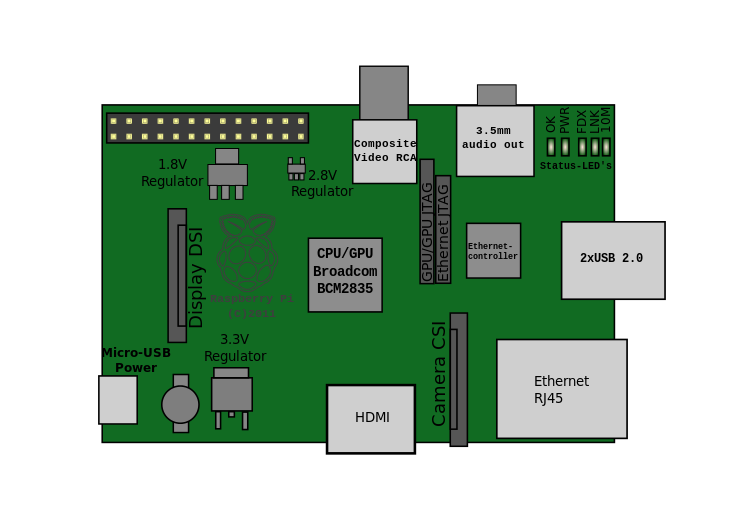
\includegraphics[width=0.5\textwidth]{raspi_pcb}
  \label{fig:raspi_pcb}
\end{figure}

\subsubsection{Broadcom BCM2835 CPU y GPU}
\subsubsection{Memoria}
\subsubsection{GPIO (Entradas y salidas de prop�sito general)}

\begin{table}
\centering
  \begin{tabular}{r r r r}
\textbf{Pin} & \textbf{Descripci�n} & \textbf{Pin} & \textbf{Descripci�n} \\
\hline
1 & \texttt{3.3v} & 2 & \texttt{5v} \\
3 & \texttt{SDA0*} & 4 & \texttt{5v} \\
5 & \texttt{SCL0*} & 6 & \texttt{GND} \\
7 &  \texttt{GPIO\_GCLK} & 8 & \texttt{TXD0*} \\
9 &  \texttt{GND} & 10 & \texttt{RXD0*} \\
11 &  \texttt{GPIO\_GEN0} & 12 & \texttt{GPIO\_GEN1} \\
13 &  \texttt{GPIO\_GEN2} & 14 & \texttt{GND} \\
15 &  \texttt{GPIO\_GEN3} & 16 & \texttt{GPIO\_GEN4} \\
17 &  \texttt{3.3v} & 18 & \texttt{GPIO\_GEN5} \\
19 &  \texttt{SPI\_MOSI*} & 20 & \texttt{GND} \\
21 &  \texttt{SPI\_MISO*} & 22 & \texttt{GPIO\_GEN6} \\
23 &  \texttt{SPI\_SCLK*} & 24 & \texttt{SPI\_CEO\_N*} \\
25 &  \texttt{GND} & 26 & \texttt{SPI\_CE1\_N*} \\
  \end{tabular}
  \caption{Descripci�n de los pines de GPIO}
  \label{table:gpio_descr}
\end{table}

\subsection{Modulo de C�mara}
\begin{figure}[h!]
  \caption{Modulo de c�mara de Raspberry Pi.}
  \centering
    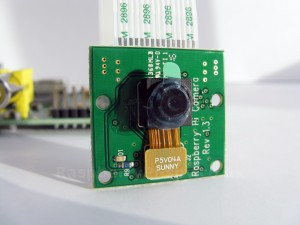
\includegraphics[width=0.5\textwidth]{raspi_camera}
  \label{fig:raspi_camera}
\end{figure}

\subsection{Software}
\section{Componentes el�ctricos, electr�nicos y electromec�nicos del Robot}
\subsection{Actuadores}
\subsubsection{Motores DC}
\subsection{Celdas 18650}
\subsubsection{Celdas Li-Ion}
\subsection{Regulador de voltaje}
\subsection{Controlador de motores DC}
Un ejemplo de funcionamiento del puente-en-H se muestra en la Figura~\ref{fig:h-bridge}, los interruptores S1, S2, S3 y S4 estan situados de tal manera que forman una letra H. \begin{figure}[h!]
  \caption{H-Bridge controlando un motor adelante y atras.}
  \centering
    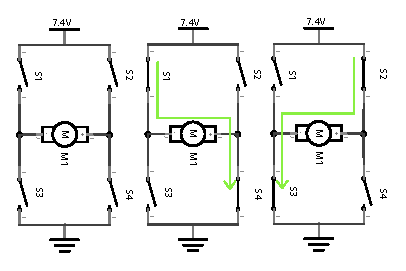
\includegraphics[width=0.4\textwidth]{h-bridge}
  \label{fig:h-bridge}
\end{figure}

\subsubsection{Puente-en-H dual L298}
El \texttt{L298} es un circuito integrado que contiene dos puentes-en-H, es decir que puede controlar dos motores al mismo tiempo. Este C.I. es capaz de controlar motores de alto voltaje y alta corriente, y acepta como entrada niveles logicos TTL.

\begin{figure}[h!]
  \caption{Empaquetado del circuito integrado L298}
  \centering
    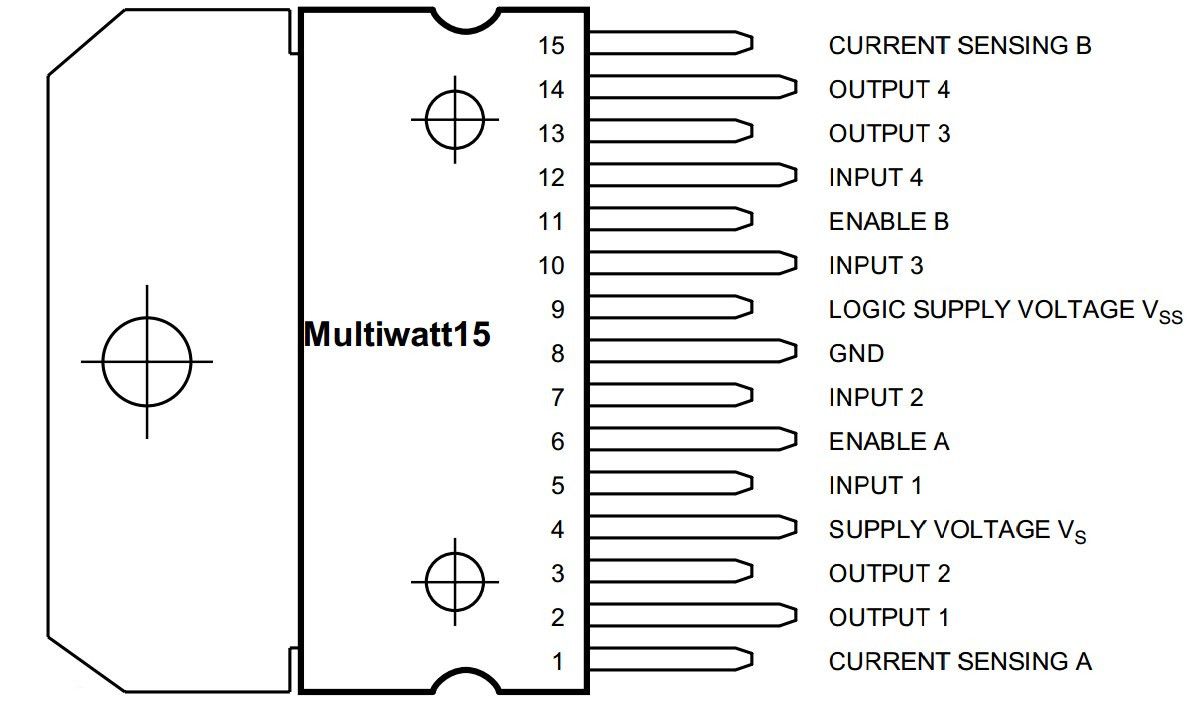
\includegraphics[width=0.4\textwidth]{hbci}
  \label{fig:hbci}
\end{figure}


%\subsection{}
%\subsection{}
\section{Partes mec�nicas del Robot}
\subsection{Tractor oruga}
\begin{figure}[h!]
  \caption{Ruedas y orugas Tamiya.}
  \centering
    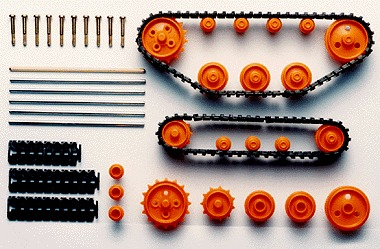
\includegraphics[width=0.4\textwidth]{oruga}
  \label{fig:oruga}
\end{figure}


\subsection{Chasis del Robot}
\subsection{Caja para celdas 18650}
%herramientas utlizadas
%descripcion de pines
%circuitos

% GPIO 18 servomotor

\chapter{Area de aplicacion}
\chapter{Metodologia}
\chapter{Conclusiones y Recomendaciones}

\begin{thebibliography}{99}
%\bibitem{Libro_ejemplo} Apellido, Nombre.Nombre texto.Editorial.A�o.# de pag
%\bibitem{PHP} PHP Web-Seite: \url{http://www.php.net}
\bibitem{robotica_wiki} Rob�tica - Wikipedia: \url{http://es.wikipedia.org/wiki/Rob�tica}. 25 de Marzo de 2014
\bibitem{opencv_wiki} OpenCV - Wikipedia: \url{http://en.wikipedia.org/wiki/OpenCV}. 25 de Marzo de 2014
\bibitem{scrum_wiki} Scrum - Wikipedia: \url{https://en.wikipedia.org/wiki/Scrum_(software_development)}. 26 de Marzo de 2014
\bibitem{opencv_oficial} P�gina oficial de OpenCV: \url{http://opencv.org/}. 27 de Marzo de 2014
\bibitem{raspberry_pi} P�gina oficial de Raspberry Pi: \url{http://www.raspberrypi.org/}. 27 de Marzo de 2014
\bibitem{raspberry_pi_wiki} Raspberry Pi - Wikipedia: \url{https://en.wikipedia.org/wiki/Raspberry_Pi}. 27 de Marzo de 2014
\bibitem{single_board_pc} Single board computer - Wikipedia: \url{https://en.wikipedia.org/wiki/Single-board_computer}. 27 de Marzo de 2014
\bibitem{reg_voltaje} Regulador de tensi�n: \url{https://es.wikipedia.org/wiki/Regulador_de_tensi\%C3\%B3n}. 11 de Septiembre de 2014
\bibitem{bateria} Bater�a de ion de litio \url{https://es.wikipedia.org/wiki/Bater\%C3\%ADa_de_ion_de_litio}. 11 de Septiembre de 2014 
\bibitem{camera_mod} Raspberry Pi camera module: \url{http://www.raspberrypi.org/products/camera-module/}. 11 de Septiembre de 2014
\bibitem{opencv_cookbook} Lagani�re, Robert.OpenCV 2 Computer Vision Application Programming Cookbook.Packt Publishing.2011.P\'agina 1
\bibitem{raspi_evilg} Norris, Donald.Raspberry Pi Projects for the Evil Genius.Mc Graw Hill.2014 . P�gina 22
\bibitem{prac_rob} Sahin, Ferat; Kachroo, Pushkin . Practical and Experimental Robotics . CRC Press . 2008 . P�gina 43
\bibitem{l298_data} STMicroelectronics . L298 DUAL FULL-BRIDGE DRIVER Datasheet. STMicroelectronics . 2000 . P�gina 2
\end{thebibliography}

\end{document}


